\section{Implementacja}
\subsection{Kontrola wersji}
Do pracy zespołowej wykorzystano narzędzie \textit{Git}. Umożliwiło ono sprawne dzielenie się zmianami w kodzie, zarządzanie i wersjonowanie zmian.

\subsection{Baza danych}
Na rysunku \ref{diagram} przedstawiony jest diagram ER schematu bazy danych.
\begin{figure}[H]
\centering
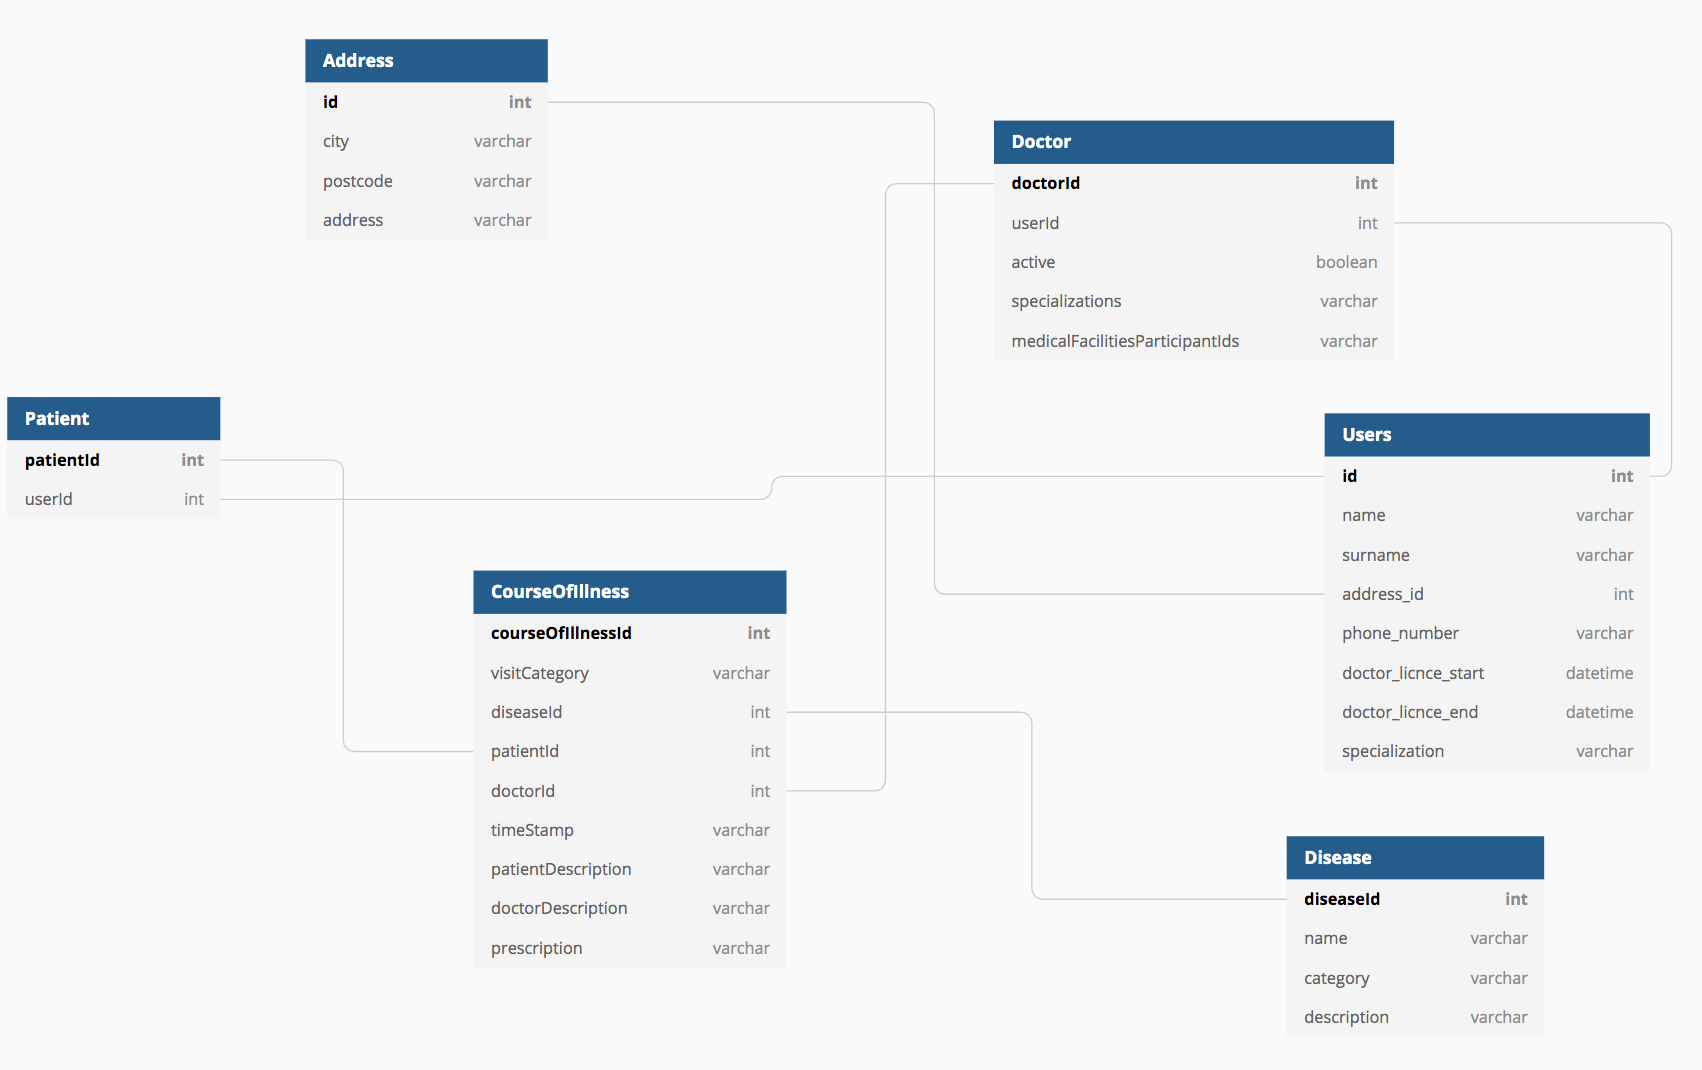
\includegraphics[width=15cm]{pictures/diagram}
\caption{Diagram ER bazy danych}
\label{diagram}
\end{figure}


Poniżej przedstawiono kod SQL wykorzystywany do inicjalizacji bazy danych:
\begin{lstlisting}[
           language=SQL,
           showspaces=false,
           basicstyle=\ttfamily,
           numbers=left,
           numberstyle=\tiny,
           commentstyle=\color{gray}
        ]
CREATE TABLE "Address" (
  "id" SERIAL PRIMARY KEY NOT NULL,
  "city" varchar,
  "postcode" varchar,
  "address" varchar
);

CREATE TABLE "Users" (
  "id" SERIAL PRIMARY KEY NOT NULL,
  "name" varchar,
  "surname" varchar,
  "address_id" int,
  "phone_number" varchar,
  "doctor_licnce_start" datetime,
  "doctor_licnce_end" datetime,
  "specialization" varchar
);

CREATE TABLE "Disease" (
  "diseaseId" SERIAL PRIMARY KEY NOT NULL,
  "name" varchar,
  "category" varchar,
  "description" varchar
);

CREATE TABLE "Doctor" (
  "doctorId" int PRIMARY KEY,
  "userId" int,
  "active" boolean,
  "specializations" varchar,
  "medicalFacilitiesParticipantIds" varchar
);

CREATE TABLE "Patient" (
  "patientId" int PRIMARY KEY,
  "userId" int
);

CREATE TABLE "CourseOfIllness" (
  "courseOfIllnessId" int PRIMARY KEY,
  "visitCategory" varchar,
  "diseaseId" int,
  "patientId" int,
  "doctorId" int,
  "timeStamp" varchar,
  "patientDescription" varchar,
  "doctorDescription" varchar,
  "prescription" varchar
);

ALTER TABLE "Users" 
ADD FOREIGN KEY ("address_id") 
REFERENCES "Address" ("id");

ALTER TABLE "Doctor" 
ADD FOREIGN KEY ("userId") 
REFERENCES "Users" ("id");

ALTER TABLE "Patient" 
ADD FOREIGN KEY ("userId") 
REFERENCES "Users" ("id");

ALTER TABLE "CourseOfIllness" 
ADD FOREIGN KEY ("diseaseId") 
REFERENCES "Disease" ("diseaseId");

ALTER TABLE "CourseOfIllness" 
ADD FOREIGN KEY ("patientId") 
REFERENCES "Patient" ("patientId");

ALTER TABLE "CourseOfIllness" 
ADD FOREIGN KEY ("doctorId") 
REFERENCES "Doctor" ("doctorId");
\end{lstlisting}


\subsection{Logika aplikacji (ang. \textit{backend})}

\subsubsection{Punkty dostępowe (ang. \textit{enpoint})}
Dzięki ogromnej popularności aplikacji internetowych opartych na języku \textit{Java} oraz \textit{framework'a Spring} możliwe było szybkie wygenerowanie dokumentacji \textit{Open API}. Pod \href{https://trunk-kartapacjentaservice.herokuapp.com/swagger-ui.html} {linkiem} dostępny jest spis wszystkich dostępnych w serwisie endpointów. Wejście w ten link będzie wymagało podania loginu i hasła (dostępnego tutaj: \ref{credentials}).

\subsubsection{Dlaczego REST?}
Zalety REST API:
\begin{itemize}
    \item Bezstanowość klienta - serwer nie ma potrzeby zapamiętywania wcześniejszego stanu, ponieważ zapytania HTTP zawierają wszystkie potrzebne informacje,
    \item Łatwość manipulowania obiektami z poziomu URL - metodami HTTP,
    \item Czytelność wykonywanych działań ze względu na używanie metod HTTP zgodnych z ich przeznaczeniem (np, DELETE do usunięcia danych, GET do pobrania),
    \item Uniwersalność odpowiedzi serwisu - możliwe jest użycie tych samych danych wygenerowanych przez serwis do obsługi aplikacji klienckich na różnych urządzeniach (np. przeglądarka i aplikacja mobilna).
\end{itemize}

\subsubsection{Zabezpieczenie danych - API}
Większość punktów dostępowych dostępnych w serwisie zabezpieczone jest przy użyciu metody \textit{Basic Auth}. Bez podania loginu i hasła niemożliwy jest dostęp do serwisu. Jedyne dostępne bez konieczności autoryzacji punkty dostępowe to te dotyczące logowania i rejestracji.

\subsubsection{Zabezpieczenie danych - baza danych}
Do zabezpieczenia danych skorzystaliśmy z symetrycznego szyfrowania. Informacje przechowywane w bazie są niemożliwe do odszyfrowania bez użycia klucza. Dane w punktach dostępowych są odszyfrowane. Odszyfrowywaniem zajmuje się aplikacja odpowiadająca za logikę serwisu.

\begin{figure}[H]
\centering
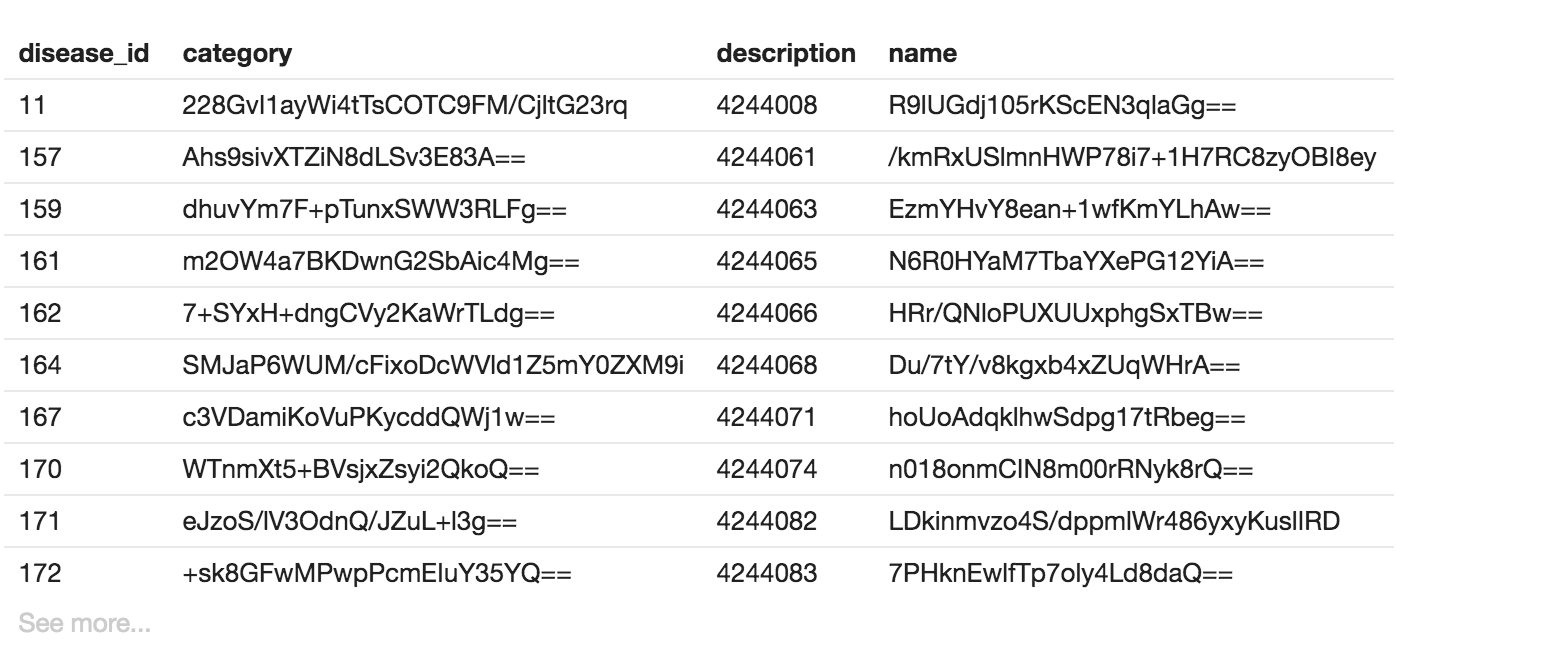
\includegraphics[width=15cm]{pictures/bd-encr}
\caption{Zaszyfrowane krotki bazy danych. Widoczne jest, że ciągi znaków zapisane w bazie danych nie są możliwe do odszyfrowania bez dekodowania.}
\end{figure}

\subsubsection{Ograniczenia}
W trakcie implementacji kolejnych funkcjonalności musieliśmy zmierzyć się z ograniczeniami serwera Heroku. Obsługa zapytań (ang. \textit{request}) jest wykonywana na ograniczonym serwerze, stąd można zaobserwować wydłużony czas oczekiwania na duże zapytanie. Skorzystanie z darmowej domeny sprawia, że funkcjonowanie strony jest po prostu wolne.

\subsubsection{Przyspieszenie}
W trakcie pierwszej wersji implementacji zastosowano wbudowany we framework Spring sterownik będący mostkiem pomiędzy obiektami programu a bazą danych. Jego zastosowanie umożliwiło stosowanie zapytań do bazy przy użyciu specjalnie spreparowanych nazw metod. Wykorzystując ten sposób i np. metodę

\begin{lstlisting}
Optional<Patient> findByUserId(Long userId);
\end{lstlisting}

automatycznie generuje się kod SQL, który odpowiada za znalezienie użytkownika o zadanym ID.

Jest to bardzo wygodne, jednak korzystając z możliwości zbudowania własnego zapytania przy użyciu języka SQL udało się uzyskać \textbf{czterokrotne} przyspieszenie związane ze stosowaniem bardziej złożonych zapytań. Wstrzyknięcie zapytania SQL zaimplementowane jest w następujący sposób:

\begin{lstlisting}
@Query(
value = "select distinct patients.patient_id, 
	my_app_users.* from my_app_users " +
	"join patients\n" +
	"on my_app_users.user_id=patients.user_id",
	nativeQuery = true)
List<PatientInfoTO> findAllPatients();
\end{lstlisting}



\subsubsection{Możliwości dotyczące rozwoju - przyspieszenie}
Przyspieszenie może zostać uzyskane np. poprzez zastosowanie architektury mikro-serwisowej, tak by każda atomowa operacja mogła zostać wykonywana niezależnie. Zapewniłoby to dużą skalowalność systemU i pod dużym obciążeniem przełożyłoby się to na przyspieszenie. 


\subsection{Warstwa wizualna aplikacji ,,Karta Pacjenta'' (ang. \textit{frontend})}
\subsubsection{Działanie warstwy wizualnej}
Warstwa wizualna oparta jest na koncepcie reakcyjnego obsługiwania zdarzeń użytkownika końcowego. Zamiast przeładowania strony po wykonaniu akcji związanej z zdarzeniem wejścia aplikacji widoku preferowane jest odświeżenie jej części.

\subsubsection{Prostota implementacji i wieloplatformowość}
Warstwa wizualna oraz warstwa serwisowa zostały oddzielone od siebie podczas implementacji - osobne repozytoria Git oraz osobne kontenery na serwerze. Rozdzielenie aplikacji w ten sposób umożliwia zapewnienie sposobu dostarczania aplikacji zgodnej z Ciągłą Integracją (ang. \textit{Continuous integration}). Umożliwia to nieprzerwane działanie aplikacji oraz odizolowuje pracę nad częścią wizualną od części logiki aplikacji. 

Podczas stylowania aplikacji wykorzystano framework Bootstrap. Obsługa akcji wykonywana jest przy użyciu frameworka Angular 7.
Frontend jest kanałem komunikacji między serwerem a klientem. Taka zależność zapewnia szybkie wykonywanie akcji
zadanych przez użytkownika bez znajomości wewnętrznej implementacji serwisu.
Podczas tworzenia "Karty Pacjenta" starano się, aby wystrój był maksymalnie przejrzysty,
wszystkie funkcjonalności opisane i rozmieszczone w jednoznaczny sposób, a komunikacja między serwerem a klientem była jak najszybsza.

\subsection{Testy obciążeniowe}

Z uwagi na to, że dostęp do aplikacji powinno mieć w tym samym czasie dziesiątki tysięcy użytkowników (pacjenci i lekarze jednocześnie).
Stąd bardzo ważną rzeczą jest obsługa endpointów, które dostarczają odpowieni zbiór danych.\\
Zaimplementowane zostały testy obciążeniowe mające na celu sprawdzenie wydajności naszego serwisu.
Skorzystaliśmy z RestTemplate, czyli biblioteki dostępnej we frameworku Spring.\\
Badane zagadnienia:
\begin{enumerate}
\item Obsługa requestów http, metod GET, POST, PUT, DELETE,
\item Weryfikacja statusów HTTP,
\item Czas odpowiedzi serwera,
\item Odporność na żądania wielu (dziesiątki tysięcy) użytkowników.
\end{enumerate}

\subsubsection{Wielowątkowość}
Wielowątkowość została zaimplementowana po to, aby możliwie najlepiej oddać realny sposób użytkowania.
W jednym momencie tysiące użytkowników może zażądać tego samego zbioru danych. Każde z urządzeń powinno zostać poprawnie obsłużone.
\subsubsection{Szybkość działania aplikacji}
Podczas przeprowadzanych testów wydajnościowych zaobserwowano spadek wydajności działania serwisu. Podczas próby pobrania przez jednego użytkownika listy wszystkich dostępnych pacjentów czas wykonania zapytania wynosił 350ms. Podczas symulowanych testów na 1000 użytkownikach próbujących otrzymać dostęp do serwisu zmierzono średni czas dostępu do pojedynczego punktu dostępowego ok. 800ms. 
\subsubsection{Rola testów w rozwoju aplikacji}
Pierwszą, dość oczywistą rolą testów, podczas tworzenia aplikacji jest weryfikacja poprawności implementacji zadań. Aplikacja, zanim zostanie przekazana klientowi powinna przejść szereg testów automatycznych jak i manualnych. Wykorzystanie dobrze napisanych testów automatycznych pozwala na zmniejszenie liczby osób (testerów), którzy odpowiedzialni są za manualne sprawdzenie poprawności działania aplikacji.

